% Tento soubor nahraďte vlastním souborem s přílohami (nadpisy níže jsou pouze pro příklad)
% This file should be replaced with your file with an appendices (headings below are examples only)

% Umístění obsahu paměťového média do příloh je vhodné konzultovat s vedoucím
% Placing of table of contents of the memory media here should be consulted with a supervisor
%\chapter{Obsah přiloženého paměťového média}

%\chapter{Manuál}

%\chapter{Konfigurační soubor} % Configuration file

%\chapter{RelaxNG Schéma konfiguračního souboru} % Scheme of RelaxNG configuration file
\chapter{Plakát}
Obrázek \ref{plakat} je zmenšený plakát, který byl vytvořen v rámci této práce. V elektronické
verzi je plakát ve formátu SVG (Scalable Vector Graphics).
\begin{figure}[p]
    \label{plakat}
    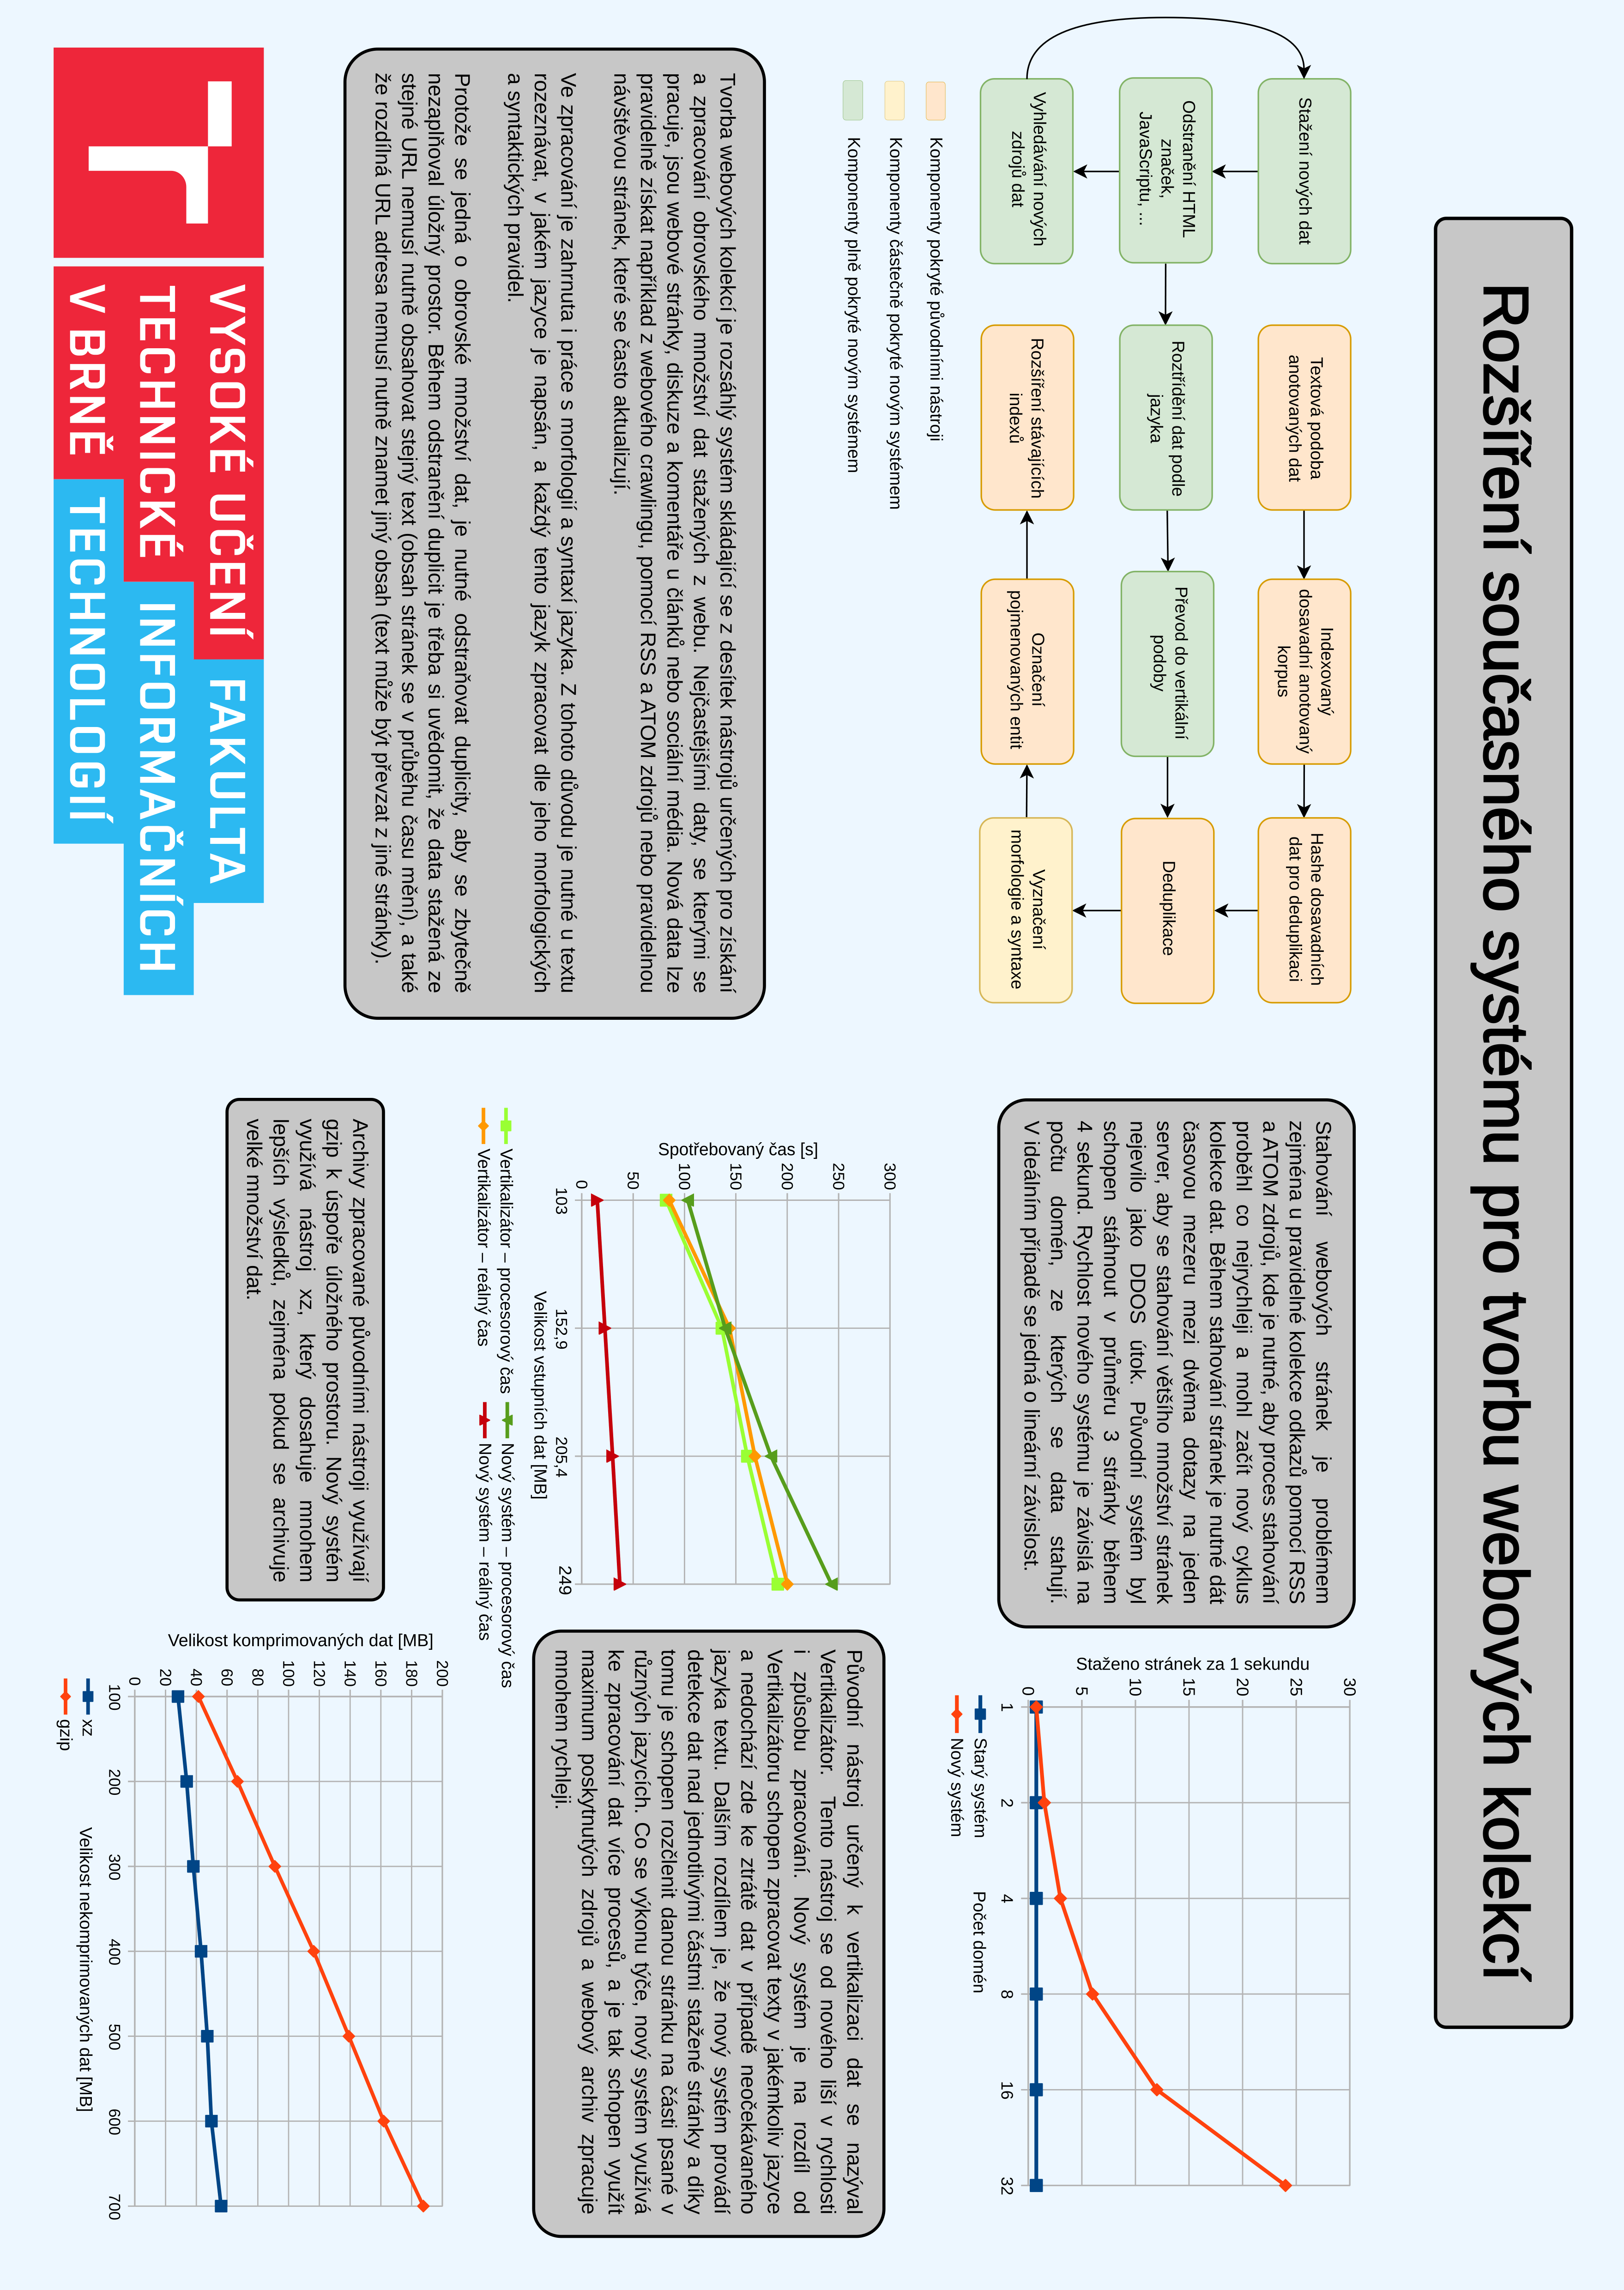
\includegraphics[height=\paperwidth,width=\paperwidth,keepaspectratio]{obrazky-figures/plakat.png}
    \caption{Plakát stručně popisující projekt.}
\end{figure}